\section{Hues} 

  Another way to represent this is with color wheels, which is much simpler and gives artists a starting point to test colors. 

  \begin{definition}[Color Wheel]
    A \textbf{color wheel} is a visual diagram derived from a set of three primary colors.   

    \begin{figure}[H]
      \centering
      \begin{subfigure}[b]{0.32\textwidth}
        \centering
        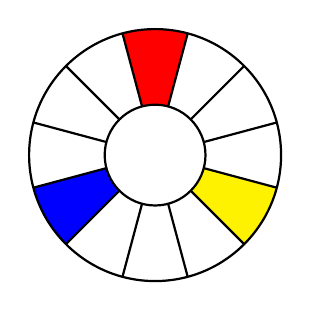
\begin{tikzpicture}[scale=0.8]
          \def\radius{2}
          
          % Complete 12-color wheel (flipped across vertical axis)
          \fill[orange!80!yellow] (0,0) -- (345:\radius) arc (345:375:\radius) -- cycle; % Yellow-Orange
          \fill[yellow] (0,0) -- (345:\radius) arc (345:315:\radius) -- cycle;         % Yellow
          \fill[lime] (0,0) -- (315:\radius) arc (315:285:\radius) -- cycle;           % Yellow-Green
          \fill[green] (0,0) -- (285:\radius) arc (285:255:\radius) -- cycle;          % Green
          \fill[teal] (0,0) -- (255:\radius) arc (255:225:\radius) -- cycle;           % Blue-Green
          \fill[blue] (0,0) -- (225:\radius) arc (225:195:\radius) -- cycle;           % Blue
          \fill[blue!50!magenta] (0,0) -- (195:\radius) arc (195:165:\radius) -- cycle; % Blue-Violet
          \fill[magenta] (0,0) -- (165:\radius) arc (165:135:\radius) -- cycle;        % Violet
          \fill[red!50!magenta] (0,0) -- (135:\radius) arc (135:105:\radius) -- cycle; % Red-Violet
          \fill[red] (0,0) -- (105:\radius) arc (105:75:\radius) -- cycle;              % Red
          \fill[red!50!orange] (0,0) -- (75:\radius) arc (75:45:\radius) -- cycle;     % Red-Orange
          \fill[orange] (0,0) -- (45:\radius) arc (45:15:\radius) -- cycle;            % Orange
          % Fill remaining sectors with white (all except 2, 6, 10)
          \foreach \i in {0,1,3,4,5,7,8,9,11} {
            \fill[white] (0,0) -- ({\i*30+15}:\radius) arc ({\i*30+15}:{(\i+1)*30+15}:\radius) -- cycle;
          }
          
          % Draw the outer circle and sector lines
          \draw[thick, black] (0,0) circle (\radius);
          \foreach \angle in {15, 45, 75, 105, 135, 165, 195, 225, 255, 285, 315, 345} {
            \draw[thick, black] (0,0) -- (\angle:\radius);
          }
          
          % Inner white circle
          \fill[white] (0,0) circle (0.8);
          \draw[thick, black] (0,0) circle (0.8);
        \end{tikzpicture}
        \caption{Primary}
        \label{fig:primary-template}
      \end{subfigure}
      \hfill 
      \begin{subfigure}[b]{0.32\textwidth}
        \centering
        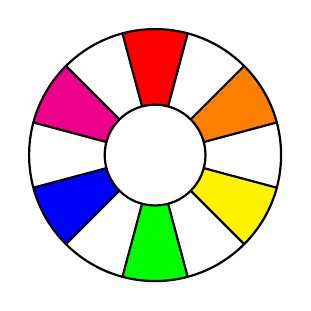
\begin{tikzpicture}[scale=0.8]
          \def\radius{2}
          
          % Complete 12-color wheel (flipped across vertical axis)
          \fill[orange!80!yellow] (0,0) -- (345:\radius) arc (345:375:\radius) -- cycle; % Yellow-Orange
          \fill[yellow] (0,0) -- (345:\radius) arc (345:315:\radius) -- cycle;         % Yellow
          \fill[lime] (0,0) -- (315:\radius) arc (315:285:\radius) -- cycle;           % Yellow-Green
          \fill[green] (0,0) -- (285:\radius) arc (285:255:\radius) -- cycle;          % Green
          \fill[teal] (0,0) -- (255:\radius) arc (255:225:\radius) -- cycle;           % Blue-Green
          \fill[blue] (0,0) -- (225:\radius) arc (225:195:\radius) -- cycle;           % Blue
          \fill[blue!50!magenta] (0,0) -- (195:\radius) arc (195:165:\radius) -- cycle; % Blue-Violet
          \fill[magenta] (0,0) -- (165:\radius) arc (165:135:\radius) -- cycle;        % Violet
          \fill[red!50!magenta] (0,0) -- (135:\radius) arc (135:105:\radius) -- cycle; % Red-Violet
          \fill[red] (0,0) -- (105:\radius) arc (105:75:\radius) -- cycle;              % Red
          \fill[red!50!orange] (0,0) -- (75:\radius) arc (75:45:\radius) -- cycle;     % Red-Orange
          \fill[orange] (0,0) -- (45:\radius) arc (45:15:\radius) -- cycle;            % Orange
          
          
          % Fill remaining sectors with white
          \foreach \i in {1,3,5,7,9,11} {
            \fill[white] (0,0) -- ({\i*30+15}:\radius) arc ({\i*30+15}:{(\i+1)*30+15}:\radius) -- cycle;
          }
          
          % Draw the outer circle and sector lines
          \draw[thick, black] (0,0) circle (\radius);
          \foreach \angle in {15, 45, 75, 105, 135, 165, 195, 225, 255, 285, 315, 345} {
            \draw[thick, black] (0,0) -- (\angle:\radius);
          }
          
          % Inner white circle
          \fill[white] (0,0) circle (0.8);
          \draw[thick, black] (0,0) circle (0.8);
        \end{tikzpicture}
        \caption{Secondary}
        \label{fig:secondary-template}
      \end{subfigure}
      \hfill 
      \begin{subfigure}[b]{0.32\textwidth}
        \centering
        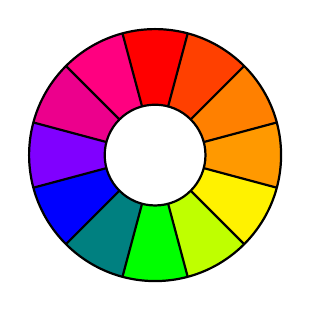
\begin{tikzpicture}[scale=0.8]
          \def\radius{2}
          
          % Complete 12-color wheel (flipped across vertical axis)
          \fill[orange!80!yellow] (0,0) -- (345:\radius) arc (345:375:\radius) -- cycle; % Yellow-Orange
          \fill[yellow] (0,0) -- (345:\radius) arc (345:315:\radius) -- cycle;         % Yellow
          \fill[lime] (0,0) -- (315:\radius) arc (315:285:\radius) -- cycle;           % Yellow-Green
          \fill[green] (0,0) -- (285:\radius) arc (285:255:\radius) -- cycle;          % Green
          \fill[teal] (0,0) -- (255:\radius) arc (255:225:\radius) -- cycle;           % Blue-Green
          \fill[blue] (0,0) -- (225:\radius) arc (225:195:\radius) -- cycle;           % Blue
          \fill[blue!50!magenta] (0,0) -- (195:\radius) arc (195:165:\radius) -- cycle; % Blue-Violet
          \fill[magenta] (0,0) -- (165:\radius) arc (165:135:\radius) -- cycle;        % Violet
          \fill[red!50!magenta] (0,0) -- (135:\radius) arc (135:105:\radius) -- cycle; % Red-Violet
          \fill[red] (0,0) -- (105:\radius) arc (105:75:\radius) -- cycle;              % Red
          \fill[red!50!orange] (0,0) -- (75:\radius) arc (75:45:\radius) -- cycle;     % Red-Orange
          \fill[orange] (0,0) -- (45:\radius) arc (45:15:\radius) -- cycle;            % Orange
          
          % Draw the outer circle and sector lines
          \draw[thick, black] (0,0) circle (\radius);
          \foreach \angle in {15, 45, 75, 105, 135, 165, 195, 225, 255, 285, 315, 345} {
            \draw[thick, black] (0,0) -- (\angle:\radius);
          }
          
          % Inner white circle
          \fill[white] (0,0) circle (0.8);
          \draw[thick, black] (0,0) circle (0.8);
        \end{tikzpicture}
        \caption{Tertiary}
        \label{fig:tertiary-template}
      \end{subfigure}
      \caption{Color wheel progression with primary and secondary colors}
      \label{fig:color-wheel-templates}
    \end{figure}
  \end{definition}

  \begin{example}[Traditional RYB]
    The \textbf{RYB} model is a subtractive color model that uses red, yellow, and blue as the primary colors. 
    \begin{figure}[H]
      \centering 
      \colorwheel{red}{yellow}{blue}{orange}{green}{violet}
      \caption{Traditional artist's color wheel using red, yellow, and blue primaries} 
    \end{figure}
  \end{example}

  \begin{example}[CMY Subtractive]
    The \textbf{CMY} model is a subtractive color model that uses cyan, magenta, and yellow as the primary colors. 
    \begin{figure}[H]
      \centering 
      \colorwheel{cyan}{magenta}{yellow}{blue}{red}{green}
      \caption{Subtractive color model used in printing} 
    \end{figure}
  \end{example}

  \begin{example}[RGB Additive]
    The \textbf{RGB} model is an additive color model that uses red, green, and blue as the primary colors. 
    \begin{figure}[H]
      \centering 
      \colorwheel{red}{green}{blue}{yellow}{cyan}{magenta}
      \caption{Additive color model used in digital displays} 
    \end{figure}
  \end{example} 

\subsection{Contrast}

  The opposite color in the color wheel has the most contrast. 


\subsection{Warm Hues} 

  \begin{example}[Warm Tones]
    \begin{figure}[H]
      \centering 
      \colorwheel{red}{orange}{yellow}{red!70!orange}{yellow!70!red}{orange!70!yellow}
      \caption{Warm-toned color wheel emphasizing reds, oranges, and yellows} 
    \end{figure}
  \end{example}

\subsection{Cool Hues}

  \begin{example}[Cool Tones]
    \begin{figure}[H]
      \centering 
      \colorwheel{blue}{teal}{purple}{cyan}{green}{violet}
      \caption{Cool-toned color wheel emphasizing blues, greens, and purples} 
    \end{figure}
  \end{example}

  \begin{example}[Monochromatic Blue]
    \begin{figure}[H]
      \centering 
      \colorwheel{blue}{blue!70!white}{blue!30!black}{blue!80!cyan}{blue!50!black}{blue!80!purple}
      \caption{Monochromatic color wheel based on blue variations} 
    \end{figure}
  \end{example}
